\documentclass[12pt,a4paper]{report}

% --- Core Packages ---
\usepackage[utf8]{inputenc}
\usepackage[english]{babel}
\usepackage{geometry}
\geometry{margin=1in, top=1.2in, bottom=1.2in}
\usepackage{graphicx}
\usepackage{amsmath, amssymb}
\usepackage{booktabs}
\usepackage{tabularx}
\usepackage{float}
\usepackage{hyperref}
\usepackage{fancyhdr}
\usepackage{lastpage}
\usepackage{refcount}
\usepackage{microtype}
\usepackage{xcolor}

% --- TikZ Package & Libraries for Native Diagrams ---
\usepackage{tikz}
\usetikzlibrary{shapes.geometric, arrows, positioning, fit, calc}

% --- Custom Colors (Navy & Ruby) ---
\definecolor{navyblue}{RGB}{0, 51, 102}
\definecolor{rubyred}{RGB}{155, 17, 30}
\definecolor{charcoal}{RGB}{45, 45, 45}
\definecolor{codebg}{RGB}{245, 245, 245}

% --- Advanced tcolorbox for Code & Output ---
\usepackage[most]{tcolorbox}
\tcbuselibrary{listings}

% Custom Code Box environment (matches page 22 of reference)
\newtcblisting{codebox}[1][Python]{
    colback=codebg,
    colframe=black,
    title=Code:,
    coltitle=white,
    fonttitle=\bfseries\small,
    arc=2mm,
    outer arc=2mm,
    left=5mm, right=5mm, top=3mm, bottom=3mm,
    boxrule=0.8pt,
    toptitle=1mm,
    bottomtitle=1mm,
    listing only,
    listing options={
        language=#1,
        basicstyle=\ttfamily\small\color{charcoal},
        keywordstyle=\color{blue}\bfseries,
        stringstyle=\color{rubyred},
        commentstyle=\color{green!50!black}\itshape,
        breaklines=true,
        showstringspaces=false,
        numbers=none
    }
}

% Custom Output Box environment (matches page 23 of reference)
\newtcolorbox{outputbox}{
    colback=codebg,
    colframe=black,
    title=Output:,
    coltitle=white,
    fonttitle=\bfseries\small,
    arc=2mm,
    outer arc=2mm,
    left=5mm, right=5mm, top=3mm, bottom=3mm,
    boxrule=0.8pt,
    toptitle=1mm,
    bottomtitle=1mm
}

% --- Hyperref Config ---
\hypersetup{
    colorlinks=true,
    linkcolor=black,
    filecolor=rubyred,      
    urlcolor=blue,
    citecolor=black,
    pdftitle={RubyAlert: Intelligent AIoT Lab Monitoring},
}

% --- Header/Footer Setup (Matches Reference Report) ---
\pagestyle{fancy}
\fancyhf{}
\setlength{\headheight}{37pt} % Accommodate BK logo

\fancyhead[L]{
    \begin{minipage}{0.08\textwidth}
        % Standard BK logo filename. Points to local hcmut.png
        
\includegraphics[width=\textwidth]{../../hcmut.png}
    \end{minipage}
    \hfill
    \begin{minipage}{0.90\textwidth}
        \footnotesize\color{charcoal}
        \textbf{University of Technology, Ho Chi Minh City}\\
        Faculty of Computer Science and Engineering
    \end{minipage}
}
\newcommand{\totalreportpages}{\pageref{LastPage}}
\newcommand{\reportfooter}{\footnotesize\color{charcoal}Multidisciplinary Project -- Academic year 2025 -- 2026\hfill Page \thepage/\totalreportpages}
\fancyfoot[L]{\reportfooter}

\fancypagestyle{plain}{%
    \fancyhf{}%
    \fancyfoot[L]{\reportfooter}%
    \renewcommand{\headrulewidth}{0pt}%
    \renewcommand{\footrulewidth}{0.5pt}%
}

\renewcommand{\headrulewidth}{0.5pt}
\renewcommand{\footrulewidth}{0.5pt}

% --- Spacing Configuration ---
\setlength{\parskip}{0.8em}
\setlength{\parindent}{0pt}

\begin{document}
\pagenumbering{gobble}

% =========================================================================
% TITLE PAGE (Replicated from page 1 of reference Report.pdf)
% =========================================================================
\begin{titlepage}
    \centering
    \vspace*{0.5cm}
    {\large\bfseries VIETNAM NATIONAL UNIVERSITY, HO CHI MINH CITY}\\[0.2cm]
    {\large\bfseries UNIVERSITY OF TECHNOLOGY}\\[0.2cm]
    {\large\bfseries FACULTY OF COMPUTER SCIENCE AND ENGINEERING}\\[1.5cm]
    
    \begin{figure}[h]
        \centering
        
\includegraphics[width=3cm]{../../hcmut.png}
    \end{figure}
    
    \vspace*{1.5cm}
    \hrule
    \vspace*{0.4cm}
    {\large\bfseries Multidisciplinary Project (CO3107)}\\[0.3cm]
    {\large Project Report - Semester 252}\\[0.5cm]
    {\Huge\bfseries ``RubyAlert: An Intelligent AIoT-Driven Laboratory Monitoring and Early Warning System''}\\[0.4cm]
    \hrule
    
    \vspace*{2.5cm}
    
    \begin{flushleft} \large
        \textbf{Instructor(s):} \quad Dr. Vo Tuan Binh \\[0.6cm]
        \textbf{Students:} \hfill \begin{minipage}[t]{0.70\textwidth}
            Le Hoang Chi Vi -- 2353336 \emph{(Group CC01, Team 29)}
        \end{minipage}
    \end{flushleft}
    
    \vfill
    {\large HO CHI MINH CITY, MAY 2026}
\end{titlepage}

\clearpage
\pagenumbering{arabic}

% =========================================================================
% LIST OF FIGURES & TABLES
% =========================================================================
\listoffigures
\addcontentsline{toc}{chapter}{List of Figures}
\newpage

\listoftables
\addcontentsline{toc}{chapter}{List of Tables}
\newpage

% =========================================================================
% TABLE OF CONTENTS
% =========================================================================
\tableofcontents
\newpage

% =========================================================================
% CHAPTER 1: INTRODUCTION
% =========================================================================
\chapter{Introduction}
\label{ch:intro}

\begin{tcolorbox}[colback=navyblue!5, colframe=navyblue, arc=1.5mm, boxrule=0.5pt, left=4mm, right=4mm, top=3mm, bottom=3mm]
    \footnotesize\color{navyblue}
    \textbf{Open-Source Project Repository:} The entire codebase, including the simulated multi-model edge server, firmware scripts, and responsive dashboard files, is hosted publicly to support academic reproducibility and collaboration: \url{https://github.com/ukulevi/rubyalert-aiot-lab}
\end{tcolorbox}

\section{Background of the Study:}
Laboratory safety represents one of the most critical aspects of academic and industrial research environments. High stress operations involving volatile solvents, pressurized gas channels, active electrical grids, and automated heaters are perpetually performed. In Vietnam, past fire anomalies and harmful chemical inhalations in research laboratories highlight the severe deficiency of proactive, autonomous safety architectures. Conventional IoT implementations are largely static, displaying telemetry on isolated physical screens or simple web views without remote control loops or natural-language interaction capacities.

The rapid rise of the \emph{Artificial Intelligence of Things (AIoT)} allows engineers to merge local microcontrollers with state-of-the-art Large Language Models (LLMs) like Google Gemini. This paradigm shifts safety monitoring from a classic passive/reactive rule-check model to a cognitive, self-governing ecosystem.

\section{Research Objectives:}
The primary objectives of this study are defined as:
\begin{enumerate}
    \item \textbf{Real-time Telemetry Collection:} Design a physical sensory node using the ESP32 to track Temperature, Humidity, and Gas/Smoke parameters via DHT22 and MQ-2 inputs.
    \item \textbf{High-Availability Dashboard:} Build a sleek Web Dashboard based on modern design systems displaying low-latency telemetry streams via WebSockets.
    \item \textbf{Bi-directional Alerting Infrastructure:} Configure a Telegram Chatbot delivering unified notifications to operators while accommodating remote control parameters.
    \item \textbf{Cognitive AI Orchestration:} Program Google Gemini AI to act as a reactive lab assistant, execute hardware configurations via Function Calling, and autonomously initiate emergency controls (e.g., fan actuation) when relative risks emerge.
\end{enumerate}

\section{Scope and Limitations}
The research parameters are structured as:
\begin{itemize}
    \item \textbf{Scope:} Deployment is confined to a singular, standard university chemistry/IoT laboratory. Actuation is simulated through a 5V relay driving a DC ventilation fan, supplemented with an active warning buzzer.
    \item \textbf{Limitations:} Messages are transmitted over the public \texttt{broker.emqx.io} MQTT Broker. Telemetry parameters are focused on relative hazard thresholds rather than absolute molecular spectrometry measurements.
\end{itemize}

% =========================================================================
% CHAPTER 2: FOUNDATIONAL KNOWLEDGE
% =========================================================================
\chapter{Foundational Knowledge}
\label{ch:foundations}

\section{Internet of Things (IoT) Architecture}
The system layout conforms to the standard three-tier IoT architectural standard:
\begin{enumerate}
    \item \textbf{Perception Layer:} Comprises the ESP32 microcontroller interfaced with the DHT22 and MQ-2 physical sensors, a 5V relay, and a piezoelectric buzzer.
    \item \textbf{Network Layer:} Uses MQTT over Wi-Fi for telemetry delivery, plus HTTPS and WSS channels for AI cloud calls and web synchronization.
    \item \textbf{Application Layer:} Entails the central Python Edge server, the Telegram Chatbot daemon, the HTML5 Web Dashboard, and the Google Gemini NLU API.
\end{enumerate}

\section{Communication Protocol Selection}
For physical-node to edge-server exchange, \textbf{MQTT (Message Queuing Telemetry Transport)} was chosen over standard HTTP due to its low header footprint (2 bytes minimum vs. kilobytes in HTTP headers), minimal network bandwidth, and native publish/subscribe messaging, which is ideal for real-time telemetry systems.

\section{Core Hardware Modules}
\begin{itemize}
    \item \textbf{ESP32 MCU:} A dual-core 32-bit CPU running at 240MHz, offering integrated Wi-Fi/Bluetooth, extensive hardware GPIO pins, and an internal 12-bit ADC essential for reading the analog voltage of the MQ-2 sensor.
    \item \textbf{DHT22 Digital Sensor:} Utilizes a capacitive humidity sensor and a thermistor to measure surrounding air, outputting a calibrated digital signal on a single-wire bus (Temperature: $-40$ to $80^\circ$C $\pm 0.5^\circ$C; Humidity: $0$-$100\%$ RH $\pm 2\%$).
    \item \textbf{MQ-2 Gas Sensor:} Features a tin dioxide ($\text{SnO}_2$) semiconductor layer. When exposed to combustible gases (LPG, Propane, CO, Methane, Smoke), the surface conductivity increases, yielding an analog output voltage directly proportional to gas density.
\end{itemize}

\section{Artificial Intelligence in IoT (AIoT)}
Rather than executing static scripts, the RubyAlert system embeds \textbf{Google Gemini AI} to introduce cognitive reasoning at the edge. By utilizing \textbf{Function Calling}, the LLM maps natural-language instructions to automated backend commands. The \textbf{3-Tier AI System Model} implemented in this work is structured as follows:
\begin{itemize}
    \item \textbf{Tier 1: Reactive Assistant:} Generates environmental audit reports and answers descriptive lab queries.
    \item \textbf{Tier 2: Agentic Actor:} Parses conversational intent and actuates relays (e.g., turning on the fan when the user states ``it feels hot in here'').
    \item \textbf{Tier 3: Autonomous Supervisor:} Evaluates early hazard escalation and autonomously acts before standard local alarms trigger.
\end{itemize}

% =========================================================================
% CHAPTER 3: SYSTEM DESIGN
% =========================================================================
\chapter{System Design}
\label{ch:design}

\section{Hardware Schematic \& Connection Specifications}
The ESP32 pin configuration is systematically mapped in Table~\ref{tab:pinout}.

\begin{table}[H]
    \centering
    \begin{tabular}{|l|l|l|l|}
        \hline
        \textbf{Component} & \textbf{Sensor Pin} & \textbf{ESP32 GPIO} & \textbf{Signal Type} \\ \hline
        DHT22 & OUT & GPIO 4 & Digital I/O \\ \hline
        MQ-2 & AO (Analog Out) & GPIO 34 & Analog Input (ADC1) \\ \hline
        Relay Module & IN & GPIO 27 & Digital Output \\ \hline
        Active Buzzer & Positive (+) & GPIO 26 & Digital Output \\ \hline
    \end{tabular}
    \caption{ESP32 Hardware Pin Connections}
    \label{tab:pinout}
\end{table}

\section{System Architecture Vector Drawing}
To represent the data pathways and physical hardware nodes within RubyAlert, Figure~\ref{fig:tikz_arch} details the complete AIoT telemetry network.

\begin{figure}[H]
    \centering
    \begin{tikzpicture}[
        node distance = 1.5cm and 1.8cm,
        block/.style = {draw, navyblue, thick, fill=navyblue!5, rectangle, rounded corners, minimum width=3.2cm, minimum height=1.2cm, align=center, font=\small},
        cloud/.style = {draw, rubyred, thick, fill=rubyred!5, ellipse, minimum width=3cm, minimum height=1.2cm, align=center, font=\small},
        arrow/.style = {thick, ->, >=stealth, charcoal}
    ]
        % Nodes
        \node [block] (esp) {\textbf{Perception Layer}\\[0.5em]ESP32 MCU \\ (DHT22 \& MQ-2)};
        \node [block, right=of esp] (mqtt) {\textbf{Network Broker}\\[0.5em]MQTT Broker \\ (\texttt{broker.emqx.io})};
        \node [block, right=of mqtt] (edge) {\textbf{Python Edge Server}\\[0.5em]Rule Engine \\ (Smart Lab System)};
        \node [block, below=of esp] (act) {\textbf{Actuators}\\[0.5em]5V Relay $\rightarrow$ Fan \\ Piezo Buzzer};
        \node [cloud, below=of edge] (gemini) {\textbf{Google Gemini AI}\\[0.5em]Function Calling};
        \node [cloud, below=of mqtt] (tele) {\textbf{Telegram Client}\\[0.5em]Bidirectional Chatbot};
        \node [block, above=of mqtt] (dash) {\textbf{Web Dashboard}\\[0.5em]Tailwind CSS / WSS};

        % Connectors
        \draw [arrow] ([yshift=2mm]esp.east) -- node[above, font=\scriptsize] {Publish} ([yshift=2mm]mqtt.west);
        \draw [arrow] ([yshift=-2mm]mqtt.west) -- node[below, font=\scriptsize, fill=white, inner sep=1pt] {Fan command} ([yshift=-2mm]esp.east);
        \draw [arrow] ([yshift=2mm]mqtt.east) -- node[above, font=\scriptsize] {Subscribe} ([yshift=2mm]edge.west);
        \draw [arrow] ([yshift=-2mm]edge.west) -- node[below, font=\scriptsize, fill=white, inner sep=1pt] {Relay command} ([yshift=-2mm]mqtt.east);
        \draw [arrow] (mqtt) -- node[left, font=\scriptsize] {WSS} (dash);
        \draw [arrow] (edge) -- node[left, font=\scriptsize] {API Call} (gemini);
        \draw [arrow] (gemini) -- node[right, font=\scriptsize] {Function} (edge);
        \draw [arrow] (edge) -- node[right, font=\scriptsize] {HTTPS} (tele);
        
        \draw [arrow] (esp.south) -- node[left, font=\scriptsize] {GPIO} (act.north);
    \end{tikzpicture}
    \caption{Vector Diagram of the RubyAlert Multi-tier AIoT Architecture}
    \label{fig:tikz_arch}
\end{figure}

\section{Centralized Edge Automation Algorithms}
To safeguard hardware integrity and ensure rapid reaction times, localized edge logic overrides cloud loops:

\subsection{Hysteresis Automation}
To relieve stress on the physical relay components caused by high-frequency switching near critical thresholds, a hysteresis band is enforced:
\begin{align}
    T_{\text{activation}} &= 35^\circ\text{C} \\
    T_{\text{deactivation}} &= 32^\circ\text{C}
\end{align}
The actuator stays active until telemetry falls below the safe deactivation limits.

\subsection{Rate of Change (RoC) Detection}
Sudden thermal spikes indicative of chemical fires are computed over localized histories:
\begin{equation}
    \text{RoC} = T_{\text{current}} - T_{t-10\text{s}}
\end{equation}
If $\text{RoC} \ge 3^\circ$C in under 10 seconds, the active buzzer and high-priority SMS notifications are immediately fired.

\subsection{Sensor Fault-Tolerance \& Hardware-Safe Fallbacks}
If a sensor is physically severed, the ESP32 intercepts empty (NaN) data. The edge server identifies this, immediately suspending automated script blocks to prevent false actuation, and activates a safe default state.

\subsection{Manual Override Priority}
To respect human authority, manual toggle commands issued via the Web Dashboard or Telegram raise a \texttt{manual\_override} flag, temporarily pausing the automatic rule engine.

\subsection{Algorithmic Flowchart}
The logic execution path of the localized edge computing platform is mapped in Figure~\ref{fig:tikz_flowchart}.

\begin{figure}[H]
    \centering
    \resizebox{0.95\textwidth}{!}{%
    \begin{tikzpicture}[
        node distance = 1.3cm,
        startstop/.style = {draw, navyblue, thick, fill=navyblue!5, rectangle, rounded corners, minimum width=3cm, minimum height=0.8cm, align=center, font=\small},
        process/.style = {draw, charcoal, thick, fill=gray!5, rectangle, minimum width=3.5cm, minimum height=0.8cm, align=center, font=\small},
        decision/.style = {draw, rubyred, thick, fill=rubyred!5, diamond, aspect=2, minimum width=3cm, minimum height=0.8cm, align=center, font=\small},
        arrow/.style = {thick, ->, >=stealth, charcoal}
    ]
        % Nodes
        \node [startstop] (start) {Start Telemetry Scan};
        \node [process, below=of start] (read) {Read Temp ($T$), Humidity ($H$), Gas ($G$)};
        \node [decision, below=of read] (fault) {Sensors Faulted?};
        \node [process, right=of fault, xshift=1.5cm] (safe) {Bypass Rules \\ Trigger SOS / Safe State};
        \node [decision, below=of fault, yshift=-0.5cm] (override) {Manual Override?};
        \node [process, right=of override, xshift=1.5cm] (bypass) {Bypass Auto-logic \\ Retain Actuator State};
        \node [decision, below=of override, yshift=-0.5cm] (limits) {$T > 35^\circ$C OR $G > 2000$ppm?};
        \node [process, below=of limits, yshift=-0.5cm] (actuate) {Actuate Fan (ON) \\ Activate local buzzer};
        \node [process, left=of limits, xshift=-1.5cm] (safe_state) {Actuate Fan (OFF) \\ Silent buzzer};

        % Connections
        \draw [arrow] (start) -- (read);
        \draw [arrow] (read) -- (fault);
        \draw [arrow] (fault) -- node[above, font=\scriptsize] {Yes} (safe);
        \draw [arrow] (fault) -- node[left, font=\scriptsize] {No} (override);
        \draw [arrow] (override) -- node[above, font=\scriptsize] {Yes} (bypass);
        \draw [arrow] (override) -- node[left, font=\scriptsize] {No} (limits);
        \draw [arrow] (limits) -- node[left, font=\scriptsize] {Yes} (actuate);
        \draw [arrow] (limits) -- node[above, font=\scriptsize] {No} (safe_state);
        
        \path [arrow] (safe.north) edge [bend right=30] (start.east);
        \path [arrow] (bypass.north) edge [bend right=35] (start.east);
        \path [arrow] (actuate.west) edge [bend left=45] (start.west);
        \path [arrow] (safe_state.north) edge [bend left=30] (start.west);
    \end{tikzpicture}%
    }
    \caption{Central Local Core Edge Algorithm Execution Flowchart}
    \label{fig:tikz_flowchart}
\end{figure}

% =========================================================================
% CHAPTER 4: METHODOLOGY AND INTEGRATION CODE
% =========================================================================
\chapter{Methodology}
\label{ch:methodology}

\section{Firmware and Server Development}
The ESP32 node is programmed using \textbf{MicroPython} for modular, rapid scripting. The central backend server is implemented in \textbf{Python 3} utilizing the Google GenAI SDK and Paho MQTT library.

An illustrative example of the centralized server-side telemetry ingest and rule engine is shown below:

\begin{codebox}[Python]
# Local Edge Rule Engine & Hysteresis Implementation
def evaluate_telemetry_rules(temp, humidity, gas):
    global fan_state, manual_override
    
    if manual_override:
        print("Manual Override active. Bypassing automation rules.")
        return
        
    # Standard thresholds
    TEMP_TRIGGER = 35.0
    TEMP_SAFE = 32.0
    GAS_TRIGGER = 2000.0
    GAS_SAFE = 1200.0
    
    # Hysteresis Automation
    if temp > TEMP_TRIGGER or gas > GAS_TRIGGER:
        if fan_state == "OFF":
            set_fan_state("ON")
            send_telegram_sos("CRITICAL: Threshold exceeded. Activating fan.")
    elif temp < TEMP_SAFE and gas < GAS_SAFE:
        if fan_state == "ON":
            set_fan_state("OFF")
            send_telegram_sos("INFO: Environment safe. Deactivating fan.")
\end{codebox}

The corresponding MQTT JSON format published by the ESP32 node is parsed as:

\begin{outputbox}
\ttfamily\small
Received telemetry on topic: rubyalert/lab\_1/telemetry\par
Payload:\par
{\normalfont\{}\par
\quad "temperature": 28.5,\par
\quad "humidity": 65.2,\par
\quad "gas": 850.0\par
{\normalfont\}}\par
Status: Environment safe. Fan state: OFF.
\end{outputbox}

% =========================================================================
% CHAPTER 5: EXPERIMENTAL RESULTS
% =========================================================================
\chapter{Experimental Results}
\label{ch:results}

\section{Visual Verification \& Dashboard Evidence}
To provide empirical evidence of the system in active runtime, the physical deployment and rendering of the Web Dashboard are demonstrated across the states shown in Figures~\ref{fig:dashboard_mqtt_connected}--\ref{fig:dashboard_gas_alert}.

\begin{figure}[H]
    \centering
    \IfFileExists{dashboard_mqttconnected_ini.png}{
        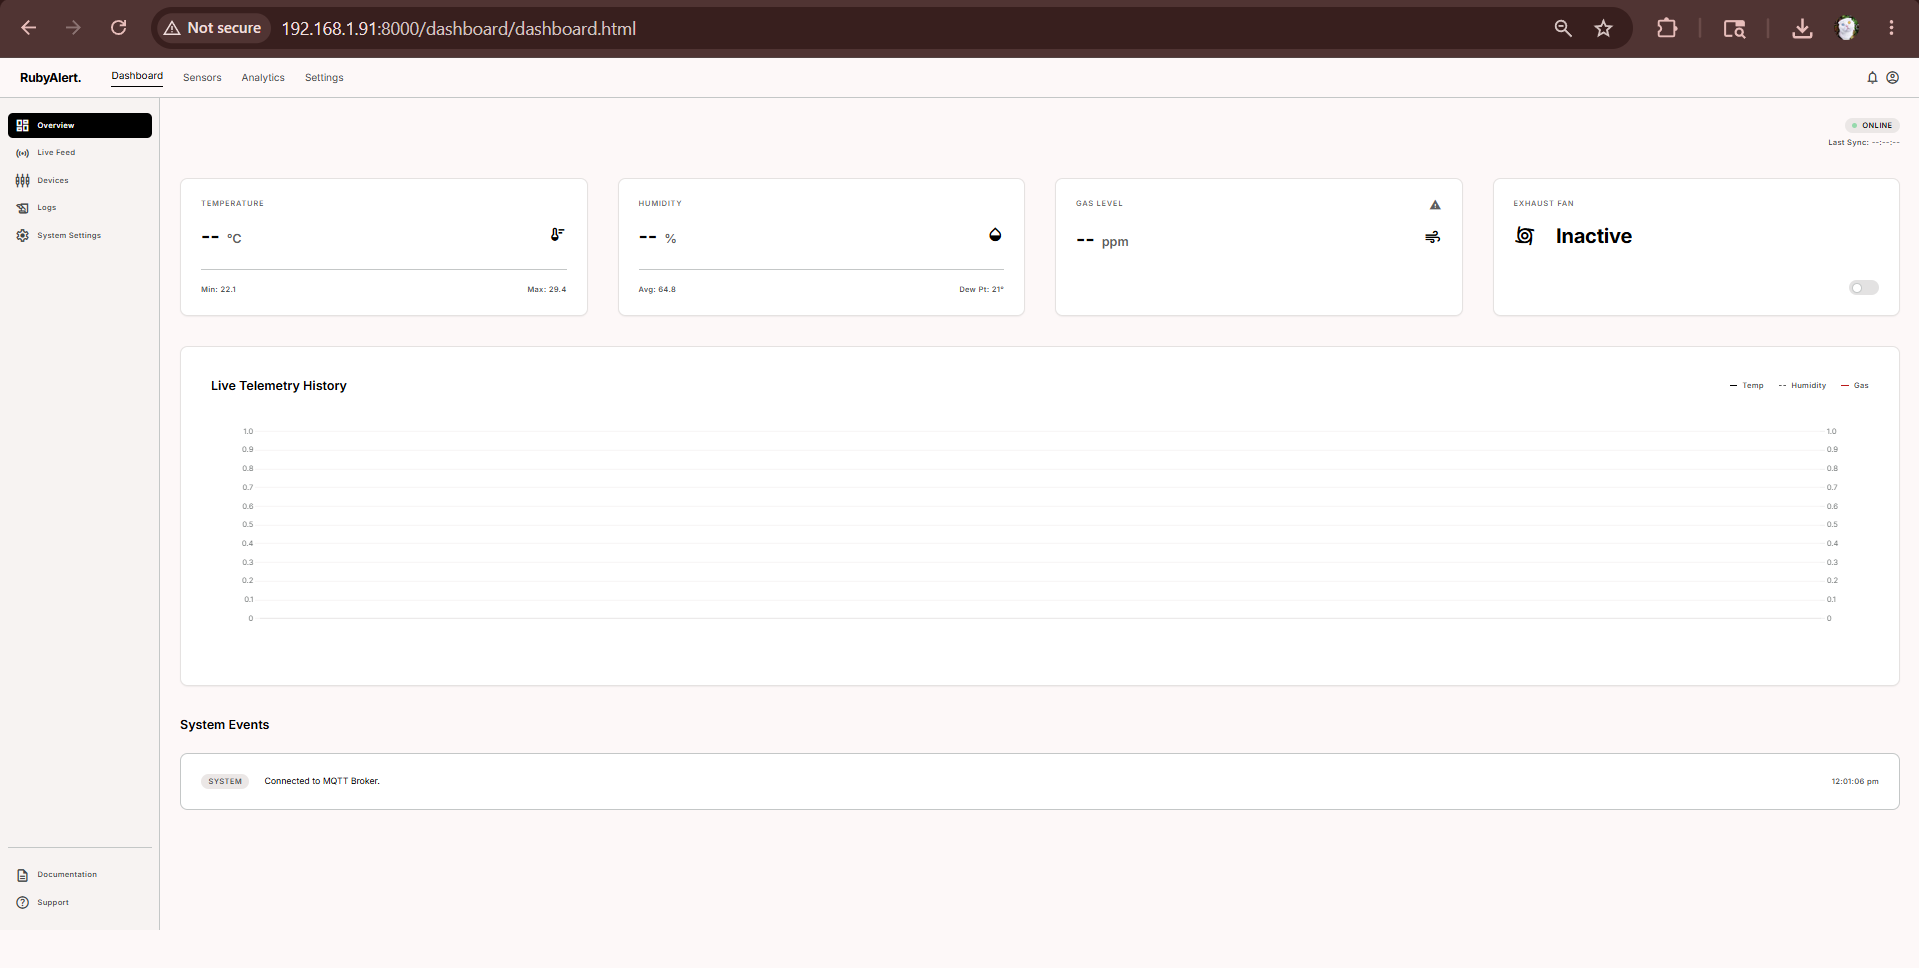
\includegraphics[width=0.95\textwidth]{dashboard_mqttconnected_ini.png}
    }{
        \begin{tcolorbox}[colback=gray!5, colframe=gray, arc=1mm, height=5cm, valign=center, halign=center]
            \bfseries\scriptsize [Initial State Placeholder]
        \end{tcolorbox}
    }
    \caption{Web Dashboard State: MQTT Connection Initialized}
    \label{fig:dashboard_mqtt_connected}
\end{figure}

\begin{figure}[H]
    \centering
    \IfFileExists{dashboard_firstdatasent.png}{
        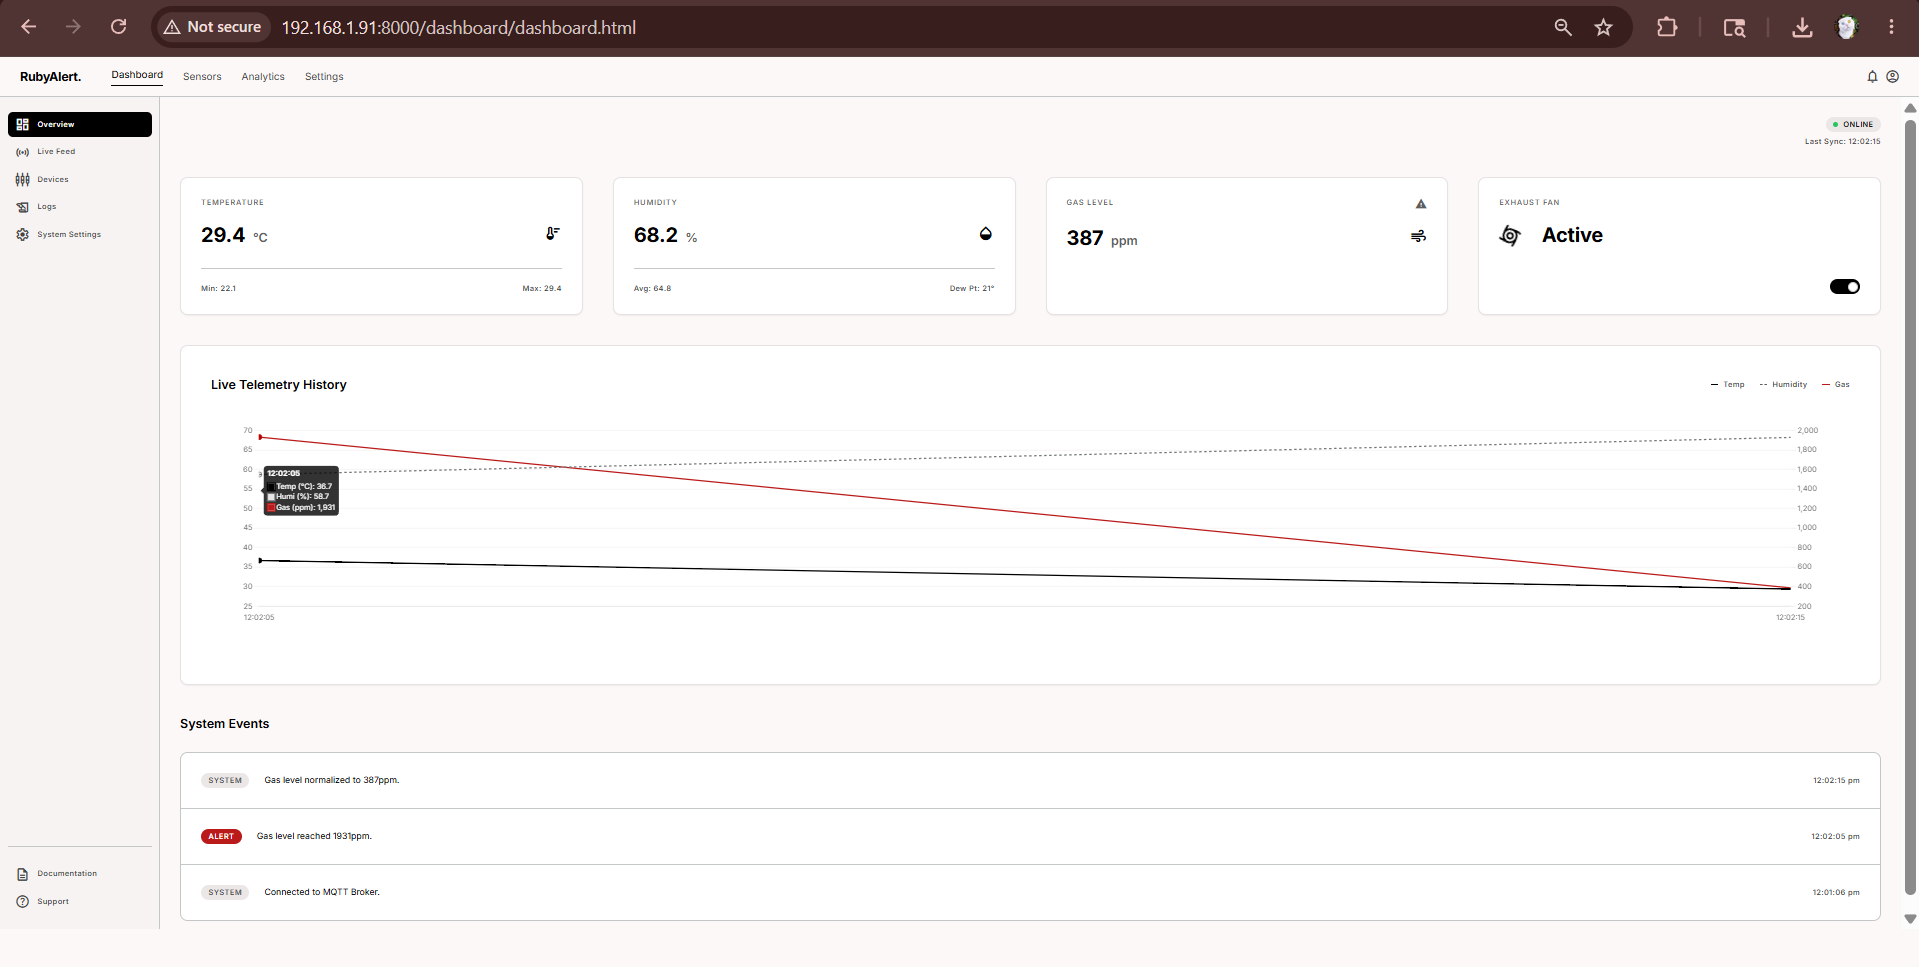
\includegraphics[width=0.95\textwidth]{dashboard_firstdatasent.png}
    }{
        \begin{tcolorbox}[colback=gray!5, colframe=gray, arc=1mm, height=5cm, valign=center, halign=center]
            \bfseries\scriptsize [Safe Steady State Placeholder]
        \end{tcolorbox}
    }
    \caption{Web Dashboard State: Normal Safe Telemetry Stream}
    \label{fig:dashboard_safe_stream}
\end{figure}

\begin{figure}[H]
    \centering
    \IfFileExists{dashboard_onecasealert_gasriskpotential.png}{
        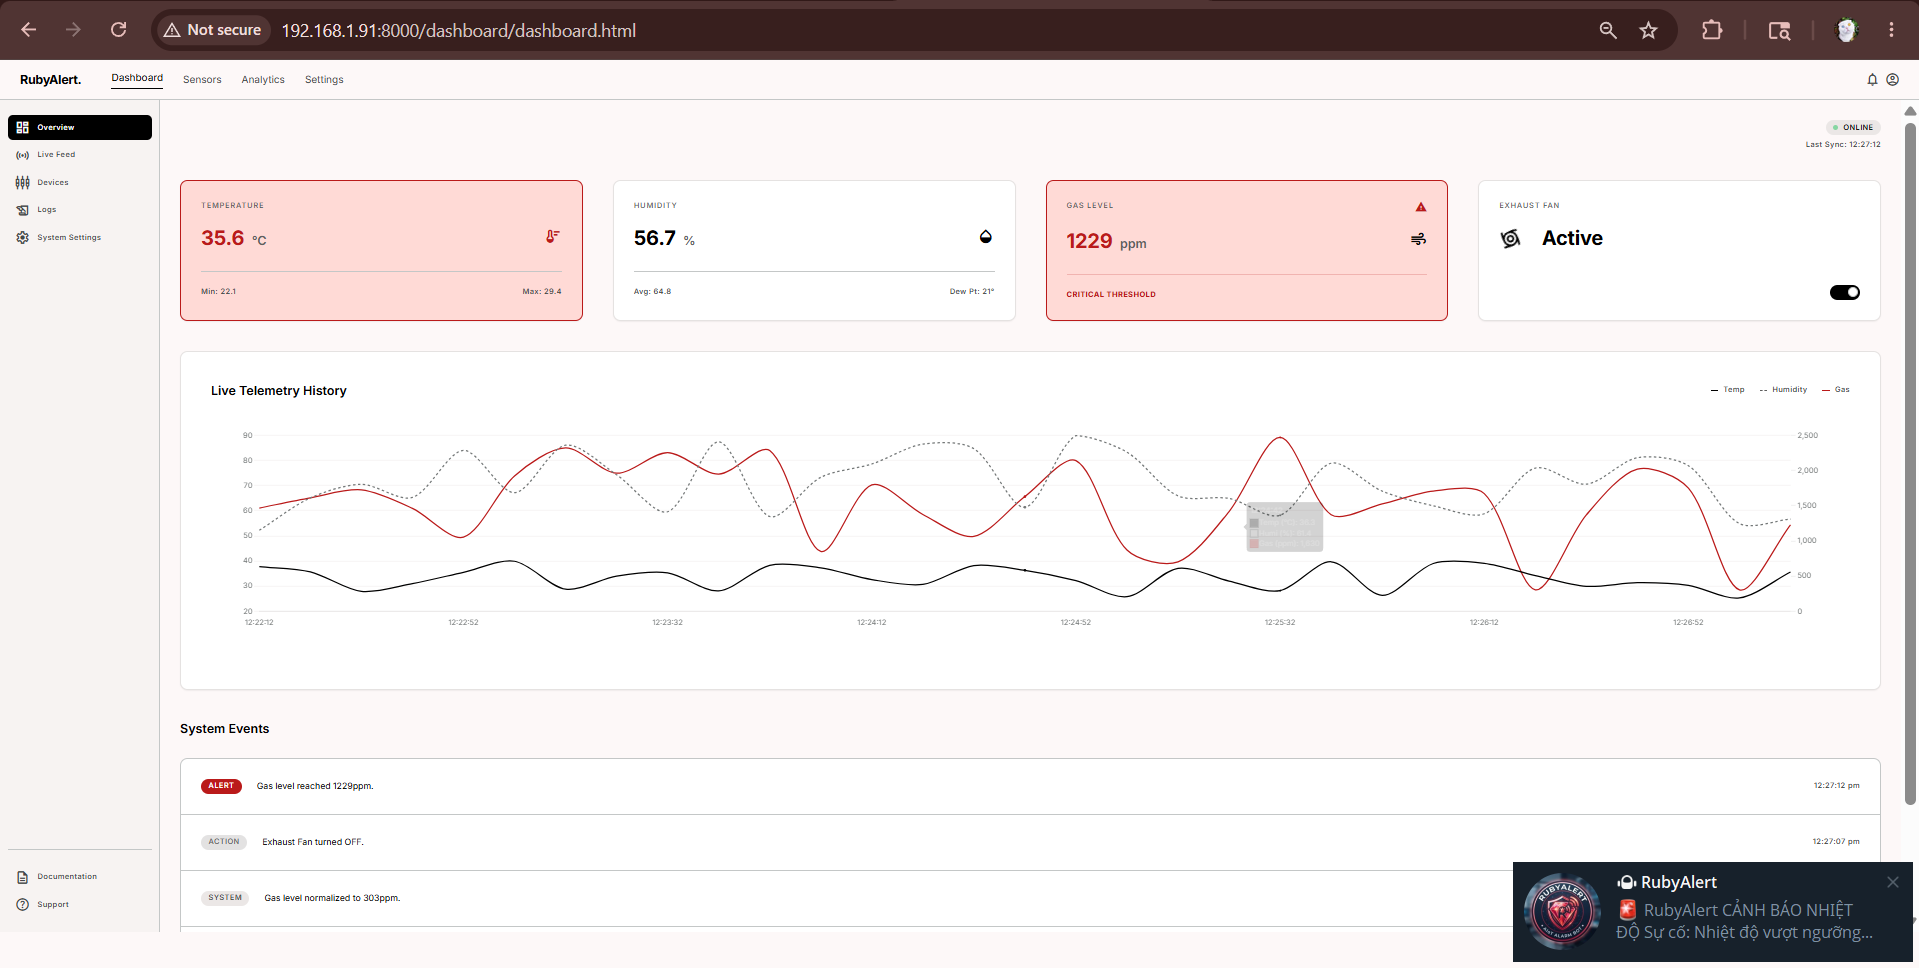
\includegraphics[width=0.95\textwidth]{dashboard_onecasealert_gasriskpotential.png}
    }{
        \begin{tcolorbox}[colback=rubyred!5, colframe=rubyred, arc=1mm, height=5cm, valign=center, halign=center]
            \bfseries\scriptsize [Leak Alert Warning Placeholder]
        \end{tcolorbox}
    }
    \caption{Web Dashboard State: Critical Threshold Breach Alert for Gas Leakage}
    \label{fig:dashboard_gas_alert}
\end{figure}


\section{Telegram Conversational Log Evidence}
The actual conversation logs captured on a mobile device illustrating bidirectional control, telemetry requests, and proactive early warning notifications are documented in Figures~\ref{fig:telegram_first_data}--\ref{fig:telegram_proactive_alerts}.

\begin{figure}[H]
    \centering
    \IfFileExists{chatbot_firstdatasent.png}{
        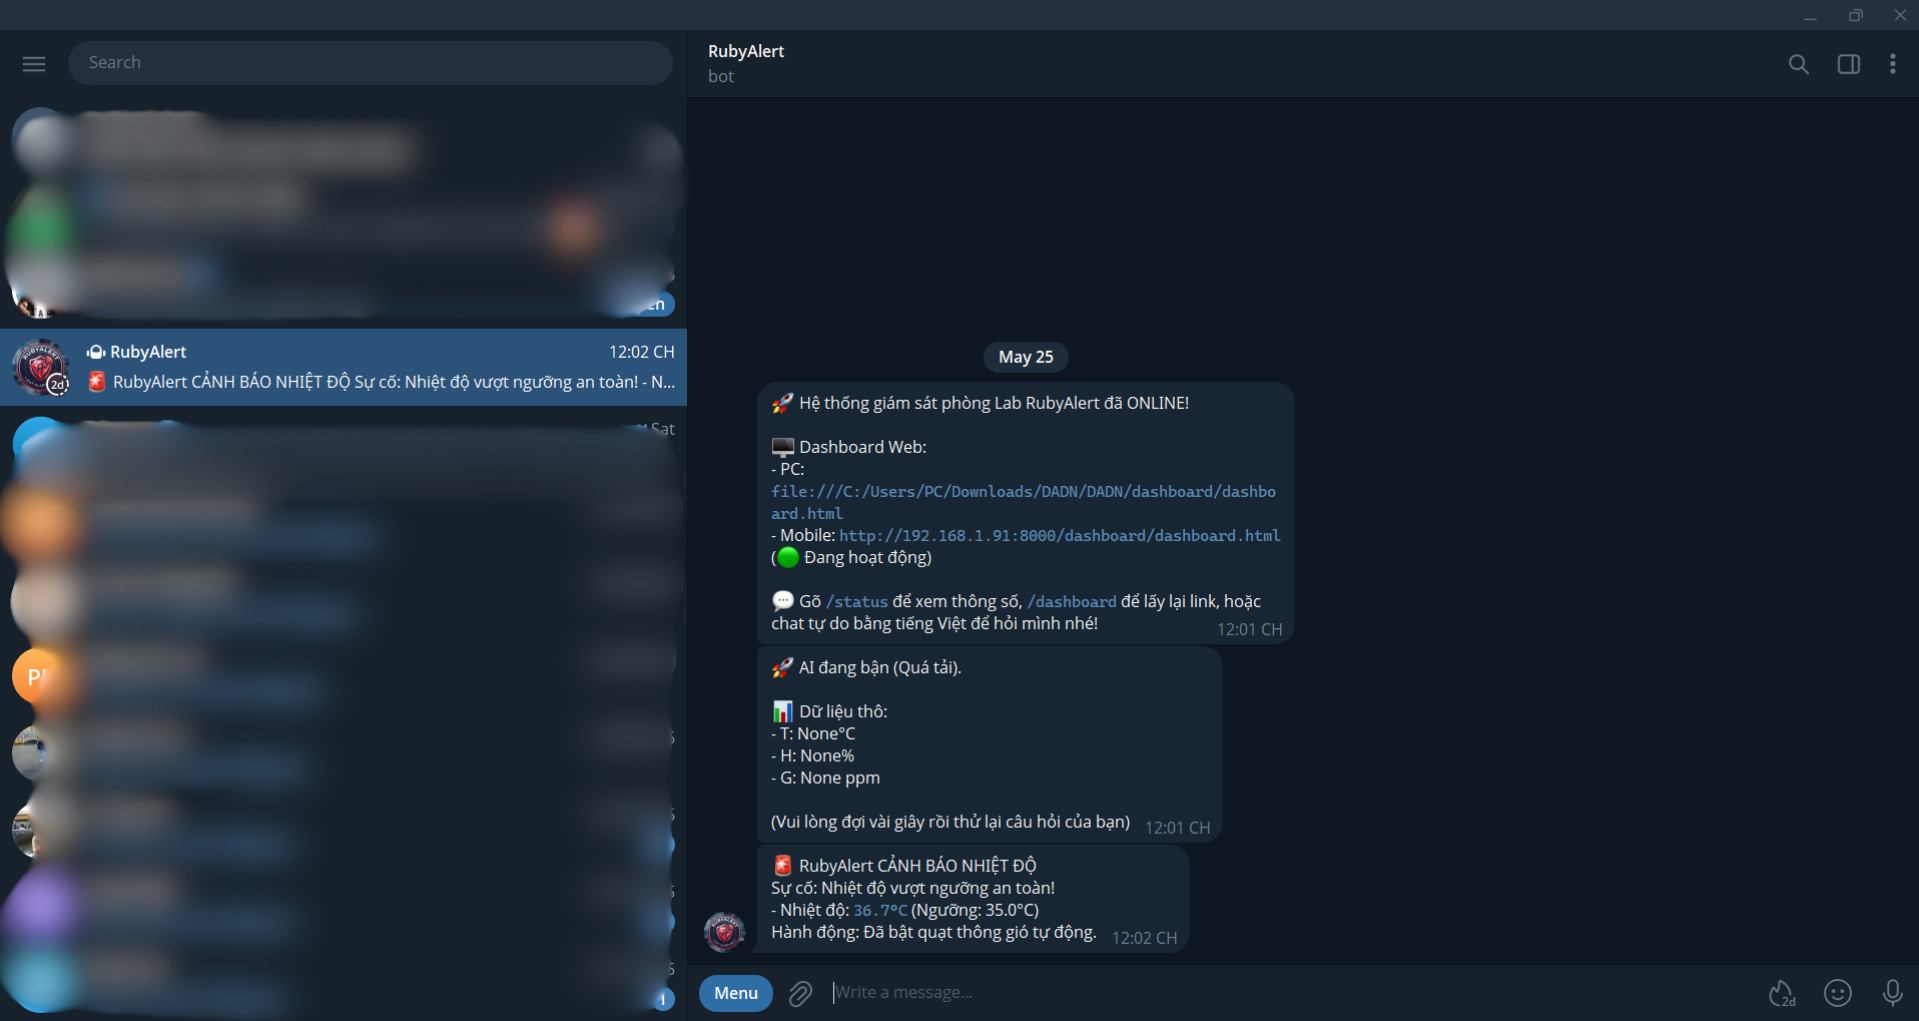
\includegraphics[width=0.95\textwidth,height=0.62\textheight,keepaspectratio]{chatbot_firstdatasent.png}
    }{
        \begin{tcolorbox}[colback=gray!5, colframe=gray, arc=1mm, height=7.5cm, valign=center, halign=center]
            \bfseries\scriptsize [Initial Chatbot Placeholder]
        \end{tcolorbox}
    }
    \caption{Telegram Chatbot Workflow: First Telemetry Stream}
    \label{fig:telegram_first_data}
\end{figure}

\begin{figure}[H]
    \centering
    \IfFileExists{chatbot_functioncall.png}{
        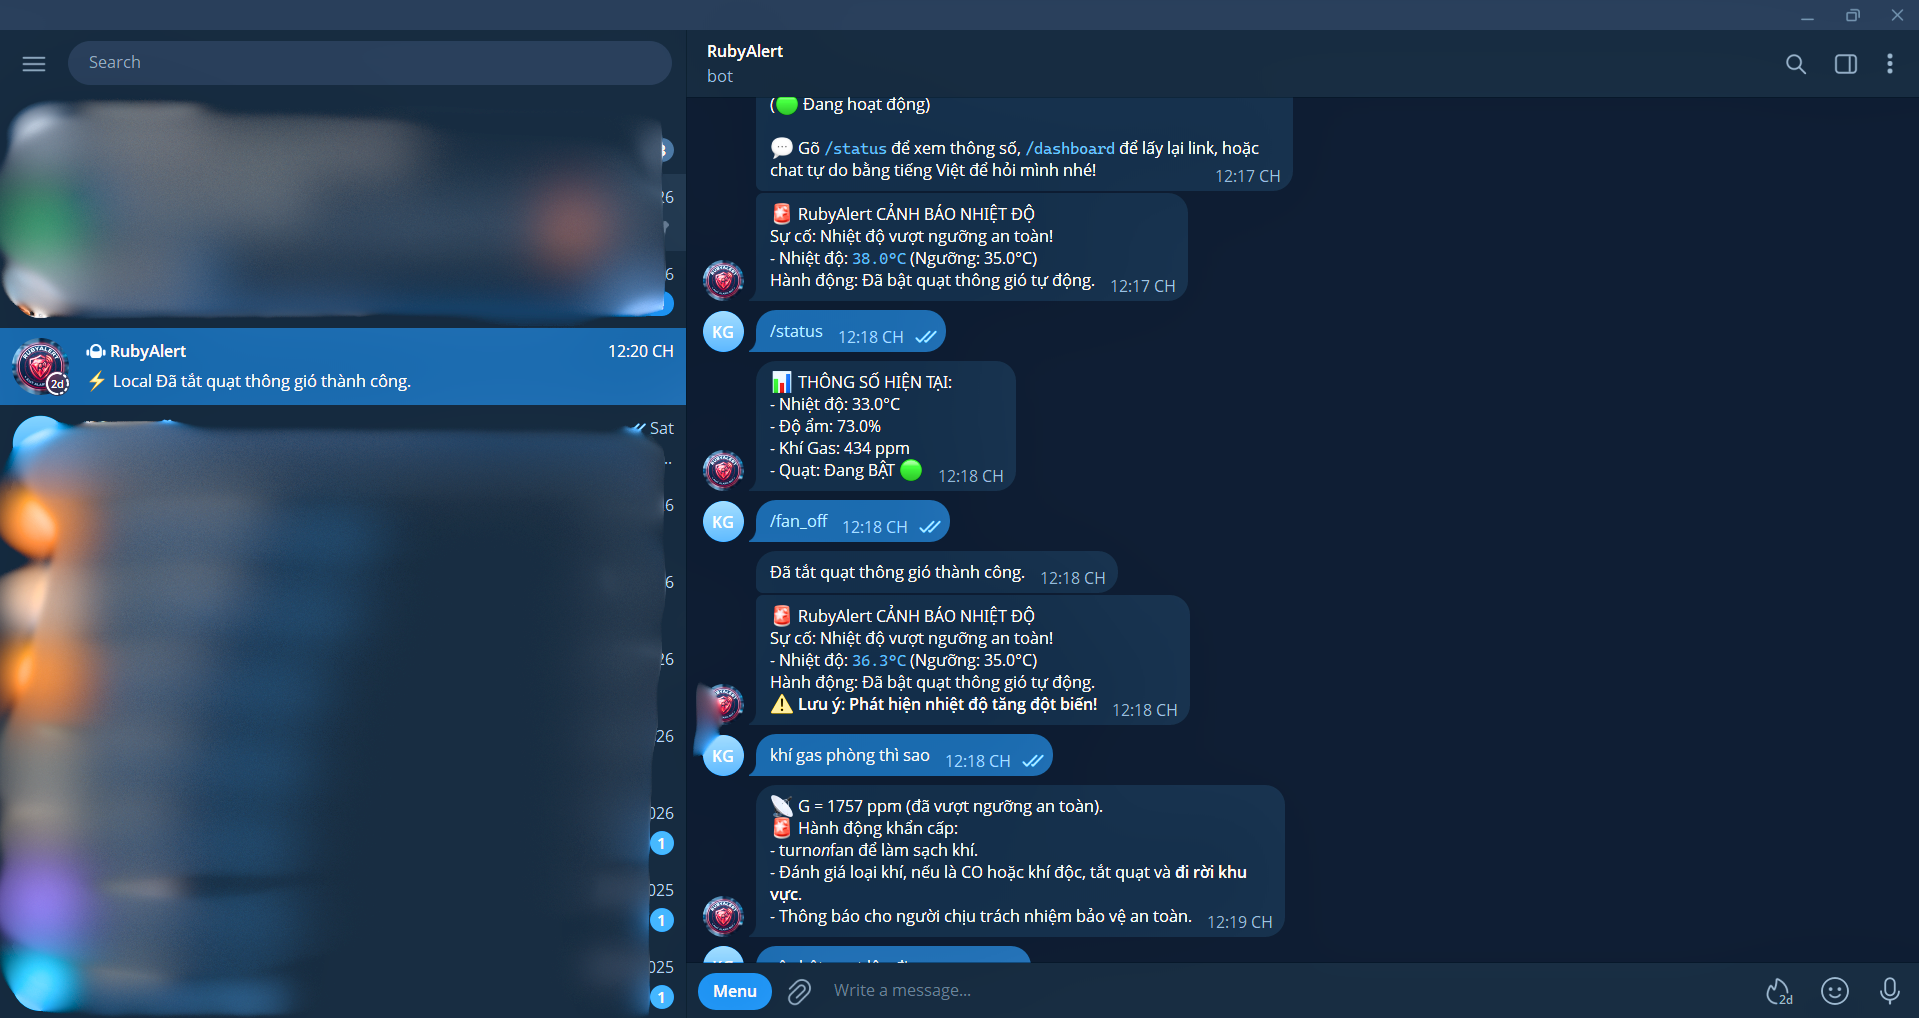
\includegraphics[width=0.95\textwidth,height=0.62\textheight,keepaspectratio]{chatbot_functioncall.png}
    }{
        \begin{tcolorbox}[colback=gray!5, colframe=gray, arc=1mm, height=7.5cm, valign=center, halign=center]
            \bfseries\scriptsize [Function Call Placeholder]
        \end{tcolorbox}
    }
    \caption{Telegram Chatbot Workflow: AI Function Calling for Device Control}
    \label{fig:telegram_function_call}
\end{figure}

\begin{figure}[H]
    \centering
    \IfFileExists{chatbot_twocasealert.png}{
        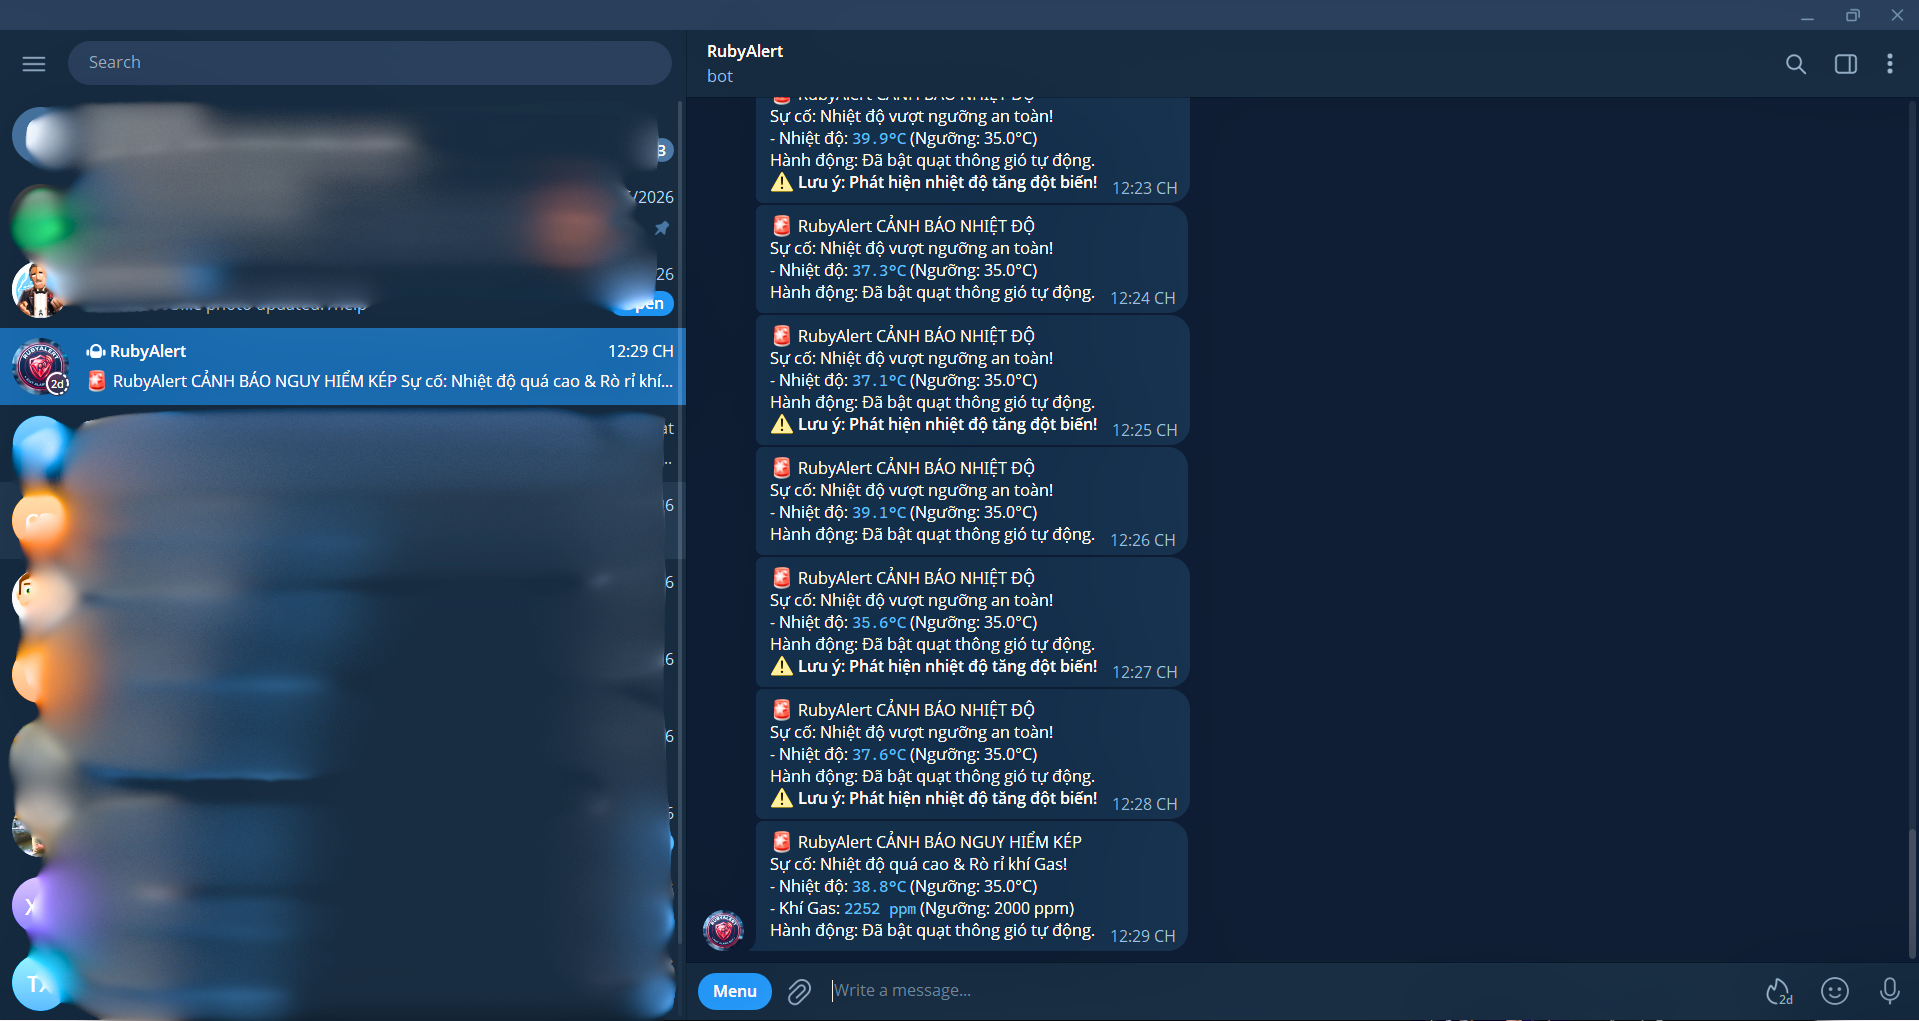
\includegraphics[width=0.95\textwidth,height=0.62\textheight,keepaspectratio]{chatbot_twocasealert.png}
    }{
        \begin{tcolorbox}[colback=rubyred!5, colframe=rubyred, arc=1mm, height=7.5cm, valign=center, halign=center]
            \bfseries\scriptsize [Proactive Warning Placeholder]
        \end{tcolorbox}
    }
    \caption{Telegram Chatbot Workflow: Proactive Warning Alerts}
    \label{fig:telegram_proactive_alerts}
\end{figure}


\vspace*{1cm}

\section{System Verification and Test Cases}
The integrated hardware and edge server were subjected to 12 rigorous evaluation scenarios. The testing results are presented in Table~\ref{tab:test_cases}.

\begin{table}[H]
    \centering
    \resizebox{\textwidth}{!}{
    \begin{tabular}{|l|l|l|l|l|c|}
        \hline
        \textbf{ID} & \textbf{Scenario} & \textbf{Action} & \textbf{Expected Response} & \textbf{Actual Response} & \textbf{Status} \\ \hline
        TC01 & Boot & Start server & Establish MQTT broker link & Connected to port 1884 & Pass \\ \hline
        TC02 & Overheat & Telemetry $T = 38^\circ$C & Fan turns ON; Telegram SOS alert & Actuator active; alert sent & Pass \\ \hline
        TC03 & Hysteresis & Telemetry $T = 33^\circ$C & Fan remains ON & Fan active (No chattering) & Pass \\ \hline
        TC04 & Cooling & Telemetry $T = 30^\circ$C & Fan turns OFF & Fan deactivated at 32C & Pass \\ \hline
        TC05 & Gas Leak & Telemetry $G = 2200$ppm & Buzzer active; Fan turns ON & Actuators fired; SOS sent & Pass \\ \hline
        TC06 & Early Leak & Telemetry $G = 1300$ppm & AI Tier 3 turns on fan & AI resolved state; Fan ON & Pass \\ \hline
        TC07 & Command & Send \texttt{/status} & Send telemetry message & Real-time stats returned & Pass \\ \hline
        TC08 & NLP command & Send ``turn on fan'' & Gemini function call set\_fan & Tool executed successfully & Pass \\ \hline
        TC09 & Filter & Send off-topic query & AI rejects prompt & Refusal prompt triggered & Pass \\ \hline
        TC10 & Report & Send \texttt{/report} & AI generates safety PDF report & Multi-paragraph PDF report & Pass \\ \hline
        TC11 & Override & Web Toggle pressed & Halts auto-rules & Manual control verified & Pass \\ \hline
        TC12 & Rate Limit & Bombard API with requests & Graceful fallback & Fallback text return & Pass \\ \hline
    \end{tabular}
    }
    \caption{RubyAlert System Verification Matrix}
    \label{tab:test_cases}
\end{table}

% =========================================================================
% CHAPTER 6: CONCLUSION AND FUTURE ROADMAP
% =========================================================================
\chapter{Conclusion}
\label{ch:conclusion}

\section{Key Contributions}
The \textbf{RubyAlert} project successfully validated that low-cost microcontrollers can be elevated into intelligent, cognitive safety platforms. The major contributions of this work are:
\begin{enumerate}
    \item \textbf{Intelligent Edge Fallbacks:} Integration of local rule-based safety controls (Hysteresis, Rate of Change) overriding cloud loops during outages.
    \item \textbf{Cognitive AIoT Architecture:} Development of a 3-tier AI system leveraging Google Gemini for reactive assistance, conversational actions, and autonomous early hazard prevention.
    \item \textbf{High-Availability Design:} Implementations of hybrid keyword/AI processing, token limits, and AI cooldowns to operate 24/7 at zero operational cost.
\end{enumerate}

\section{Future Roadmap}
Future extensions of the RubyAlert platform will focus on:
\begin{itemize}
    \item \textbf{Private Broker Security:} Transitioning to a local Mosquitto MQTT Broker equipped with TLS/SSL encryption and password security.
    \item \textbf{Persistent Logging:} Integrating an InfluxDB database to store telemetry histories for long-term regression modeling.
    \item \textbf{On-board Diagnostics:} Wiring a physical SSD1306 OLED screen to the ESP32 to display sensor stats during network disconnections.
\end{itemize}

% =========================================================================
% REFERENCES
% =========================================================================
\begin{thebibliography}{9}
    \bibitem{gemini}
    Google Gemini API documentation, Available online: \url{https://ai.google.dev/docs}.
    
    \bibitem{mqtt}
    OASIS Standard, MQTT Version 5.0, Available online: \url{https://mqtt.org/}.
    
    \bibitem{esp32}
    Espressif Systems, ESP32 Technical Reference Manual, Available online: \url{https://espressif.com/}.
    
    \bibitem{rubyalert-repo}
    Le Hoang Chi Vi, RubyAlert AIoT Laboratory Monitoring and Warning System Source Code, GitHub Repository, 2026. Available online: \url{https://github.com/ukulevi/rubyalert-aiot-lab}.
\end{thebibliography}

\end{document}
